\chapter{Background and History\label{section:history}}
\section{Background}\label{section:background}
In this section we will cover all the necessary information to understand this
Thesis. We will start on a high level and slowly delve deeper into the
intricacies of a camera.

\subsection{Camera}
Before we delve deeper, what is a camera? This section covers a brief
and incomplete history of cameras followed by an explanation of how modern
cameras work based largely on the book~\cite{hammond1981camera}. In the
simplest of terms, a camera is just a box with a tiny hole. This box with the
tiny hole is called the \textit{Camera Obscura}, which is a natural phenomenon
where light enters a small hole into a dark box the light will be projected
upside down to the opposing wall. This discovery goes back to the Chinese
philosophers of the fifth century BC. The first record of seeing an inverted
image when looking through a pinhole was by the philosopher Mo Ti~(aka. Mozi).
This was the very basics of a camera, it was another four centuries before Tuan
Chheng Shih took another crack at this. He realized that the image was inverted
because, like an oar that is attached to a boat; when the oar is up, the blade
is down. In the west, Aristotele had also seen this phenomenon. Observations
made by the Chinese and the Greek are very close, to the extent that it is
unclear if they were made independently or if there was collaboration. In
\cref{fig:cameraobscura} we can see an example of how this system looks like.
The light comes and flips it around. This is the basis of cameras.

Jumping ahead to the 13th century, Roger Bacon began working with the Camera
Obscura. He described a way to create an aerial image using a mirror in front of
the aperture\footnote{The hole in the "camera".} so that an observer would not
see anything. For example to view on people walking underneath a window.

This was only the first part though, by the 18th century people had largely
figured out what Camera Obscuras were. Lenses existed to create a clearer
projected view. The part that was left was to actually store the light onto
something. In 1725 Johann Heinrich Schulze observed that when silver salts
were exposed to light, they darkened. Contrary to what people believed at the
time he showed that it was due to light alone, not the air or the
sun~\cite{gernsheim1986concise}. After much experimentation based on this
discovery, a French inventor named Nic\'ephore Ni\'epce figured out how to
then capture an image. This image was the view of his window taken onto a
pewter plate~\cite{gernsheim1986concise}. Today silver chloride is no longer
used in cameras, we do not need to produce negatives of images to produce an
image. Instead we use photodiodes, these are diodes that can convert light to
current. We will cover modern sensor technologies in \cref{section:sensortechnology}.

Finally in 1826 Joseph Nic\'ephore Ni\'epce captured the first image (see
\cref{fig:worldsfiristimage}) using a sliding box. So how do all of these tie
into modern cameras? The mirror design that Roger Bacon designed is now in use
in devices such as DSLRs when using the viewfinder window. When pressing down
the shutter button, the mirror flips down which is why when taking a picture the
viewfinder goes blank for a bit. This allows the sensor to receive light, which
the photodiodes then turn into electricity. After the sensor receives light, it
gives the image data to the \textit{Image Signal Processor} (ISP), the ISP is
covered in detail in \cref{section:isp}. DSLRs also often provide a digital
viewfinder, in this case the optical viewfinder is bypassed and the light is
provided to the sensor instead. The ISP then processes this image and spits out
a lower quality image for preview. As mobile phones do not have optical
viewfinders, this is what mobile phones then use.

\begin{figure}
    \centering
    \subfloat[Camera Obscura]{
        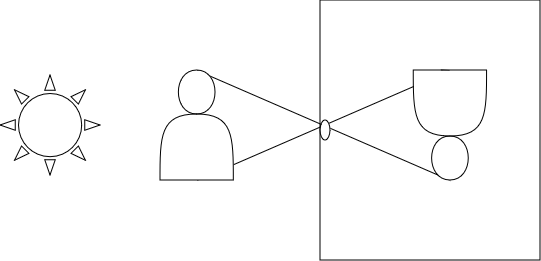
\includegraphics[width=0.5\textwidth]{figures/camera obscura.png}
        \label{fig:cameraobscura}
    }
    \subfloat[Worlds first image~\cite{gernsheim1986concise}]{
        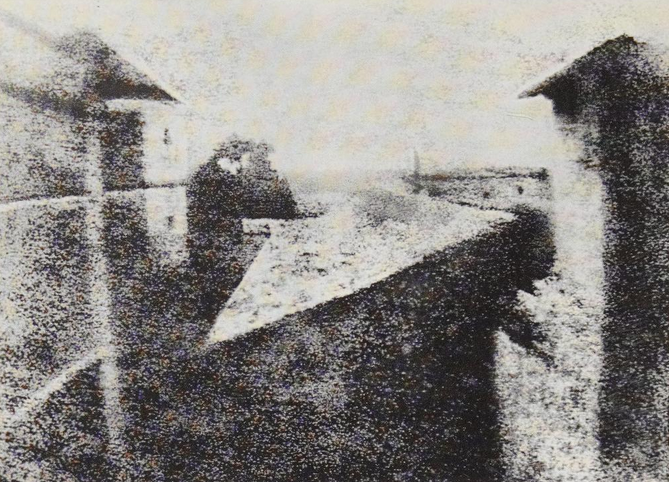
\includegraphics[width=0.4\textwidth]{figures/worldsfirstimage.png}
        \label{fig:worldsfiristimage}
    }
    \qquad
    \subfloat[A DSLR camera]{
        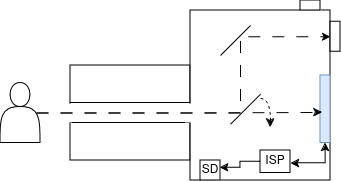
\includegraphics[width=0.4\textwidth]{figures/camera.png}
        \label{fig:camera}
    }
    \caption{}
\end{figure}


\subsection{3D Cameras}\label{section:3Dcameras}
In fields like robotics 3D cameras are used, this allows the robots to get a
sense of depth. There are many different technologies that are used for getting
depth, such as \textit{Light Detection And Ranging}
(LiDAR)~\cite{henley23lidar}, stereo cameras and more. We will give a brief
overview of how some of these technologies work.

\textbf{LiDAR} as the name suggests, works using light ($c$), specifically
lasers. It measures distance ($d$) by measuring the time ($t$) it takes for the
light to travel to the object and back.
\[
    d = \frac{c \cdot t}{2}
\]
If the laser hits for example a mirror, an object that reflects the light
elsewhere, the distance measurement may be inaccurate. There is some work that
has been done in order to improve the accuracy of measurements on these
surfaces~\cite{foster2013visagge, henley23lidar}. While the technology has come
a long way, often a secondary sensor technology is accompanied with LiDAR for
detecting specular surfaces such as ultrasonic scanners~\cite{diosi2004advanced}.

\textbf{Stereo cameras}, like human eyes uses two cameras next to each other.
By taking two images depth can be calculated~\cite{adi2017distance}. It is done
by finding the same point in the two images, which is a well known problem~\cite{scharstein2002taxonomy}.
There are several solutions to this problem,
a simple one is the absolute difference in color. While we will not delve
deeper into the algorithms here, a detailed comparison can be read from~\cite{scharstein2002taxonomy}.

\subsection{Sensor Technology}\label{section:sensortechnology}
At its core, sensors are just some photodiodes that can convert photons into
electrical charge. In this section we will cover how the two common sensor type
perform this conversion.

There are multiple types of photodiodes, though the idea behind them is to
create voltage out of photons that hit them. It does this using a
\textit{positive-negative} (PN) junctions, a junction made of one positive and
one negative material that do not fill all of the electron slots in the atom.
This allows electrons to then flow freely, allowing the charge to
move~\cite{peterson2001works}.

\begin{figure}
    \centering
    \subfloat[CCD blooming effect,\\\textit{image source: \href{https://en.wikipedia.org/wiki/Charge-coupled\_device}{Wikipedia}}]{
        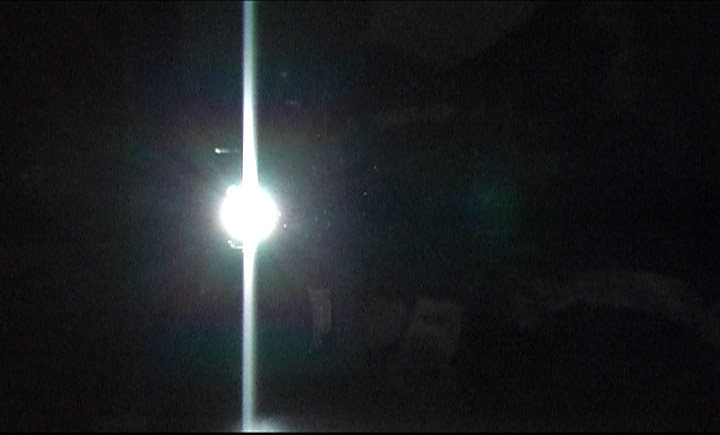
\includegraphics[width=0.40\textwidth]{figures/ccd_blooming.jpg}
        \label{fig:ccdbloom}
    }
    \subfloat[CMOS vs CDD comparison~\cite{ieeeCMOS}]{
        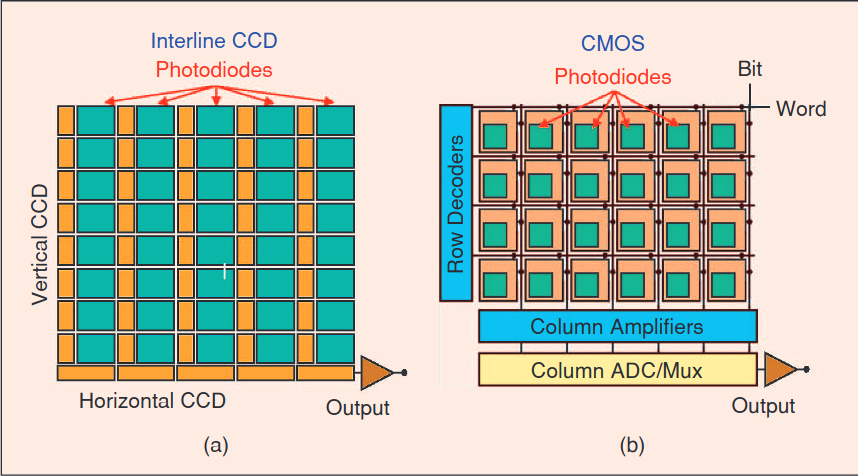
\includegraphics[width=0.5\textwidth]{figures/cmos_vs_cdd}
        \label{fig:cmosvsccd}
    }
    \caption{}
\end{figure}

\subsubsection{Complementary Metal Oxide Semiconductor Sensors}
\textit{Complementary Metal Oxide Semiconductor} (CMOS) sensors are very old
sensors, being around since the 1960s~\cite{ieeeCMOS}. Over the years due to
lithography improvements they have become very good, being able to compete with
with \textit{Charged Couple Device} (CCD) sensors which are known for better
image quality technology~\cite{ieeeCMOS}. While CCDs have a better image quality, it requires
much more power than CMOS which can be up to 100 times less power hungry~ \cite{CMOSReview}.
This means that in many mobile devices and other low power
devices prefer CMOS over CCDs.

CMOS sensors are similar to the CMOS memory chips, unlike the memory chips the
sensors use photodiodes along with amplifiers (\cref{fig:cmosvsccd}) over
transistors. The amplifiers exist to, well, amplify the signal. This design
allows us to access individual pixels quickly, see \cref{fig:ccdbloom} using
random access on top of being able to read out R, G and B signals
simultaneously~\cite{cmosAlen}. Because there are so many photodiodes along
with amplifiers, electrical fluctuation is created. This causes intermittencies
in the quality of the image, there are a number of noise reduction algorithms
that can be applied on the image to remove these.

Curious readers can have a look at~\cite{CMOSReview, ieeeCMOS} for a more
in depth overview of what CMOS sensors are.

\subsubsection{Charged Couple Device Sensors}
\textit{Charged Couple Device} (CCD) sensors were for a long time considered
significantly better than CMOS~\cite{ieeeCMOS}. It works using capacitors next
to the photodiodes to create voltage out of charge which is then read out in a
serial manner. Unlike CMOS, CCD allows you to design very small pixel sizes as
the pixels themselves do not require much real estate. The downside of this is
that this creates a lot of heat, requiring good cooling~\cite{meng2016numerical}
which is not always available in devices such as mobile phones. In
\cref{fig:cmosvsccd} we can see how the CCD sensor looks like on a high level.
Because CCD sensors read the signals row by row, if there are some pixels are
very bright it can create visual effects for the entire row~\cite{ieeeCMOS} as
can be seen in \cref{fig:ccdbloom}.


\subsection{Image Formats} \label{section:imageformats}
There are a number of different image formats, their purpose is to store an
image in an efficient way. We will cover some common ones, while the list is
not conclusive it will serve as a good base. We will cover two raw formats and
one encoded format.

\begin{wrapfigure}{r}{0.4\textwidth}
  \centering
  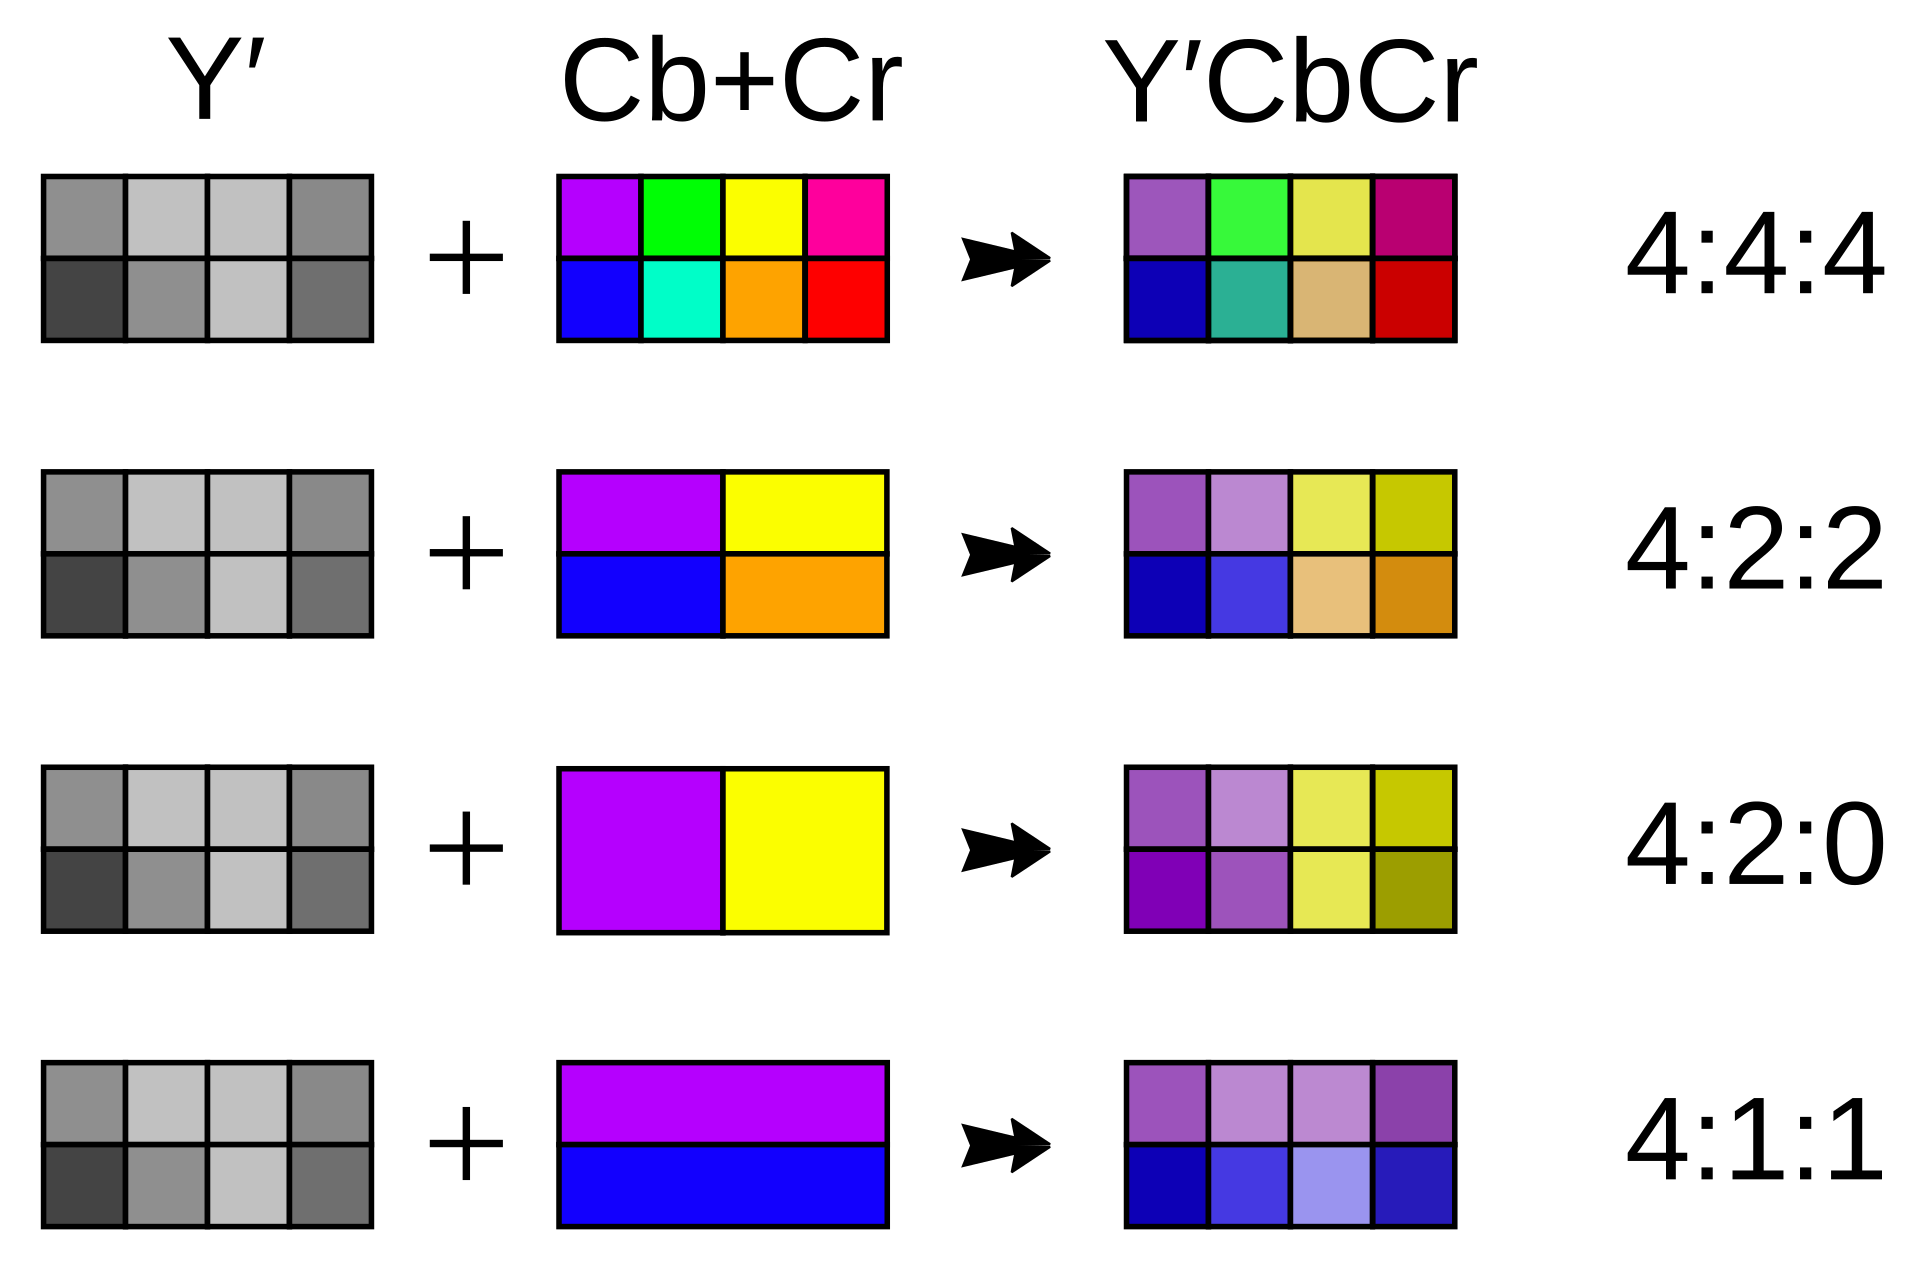
\includegraphics[width=0.35\textwidth]{figures/ycbcr.png}
  \caption{YCbCr chrominance encoding, \textit{image source: \href{https://en.wikipedia.org/wiki/Chroma_subsampling}{Wikipedia}}}
  \label{fig:ycbcr}
\end{wrapfigure}
\textbf{YCbCr} (aka. YUV) is based on three components: Y is for luminance, i.e., the
brightness, Cb is the blue-chrominance, Cr is the
red-chrominance~\cite{safir2022rgb}. YCbCr is clever, as the human eye can see
more luminance than chrominance, it takes this into account in the
encoding process. The different ways to encode YCbCr is described in the
"A:B:C" notation, which describes how the Cb and Cr sampled in relation to the
Y component. In \cref{fig:ycbcr} we can see different ways chrominance is
encoded

\pagebreak
\textbf{RGB} similarly to YCbCr is based on three components: Red, Green, and
Blue. There is also an optional channel, the alpha channel A which describes
how transparent the color is. RGB can be converted to and from YCbCr in the
following way~\cite{yang2007ycbcr}:

\[
\begin{bmatrix}
Y \\
Cb \\
Cr
\end{bmatrix}
=
\begin{bmatrix}
0.299 & 0.587 & 0.114 \\
-0.169 & -0.331 & 0.499 \\
0.499 & -0.418 & -0.0813
\end{bmatrix}
\begin{bmatrix}
R \\
G \\
B
\end{bmatrix}
+
\begin{bmatrix}
0 \\
128 \\
128
\end{bmatrix}
\]

\[
\begin{bmatrix}
R \\
G \\
B
\end{bmatrix}
=
\begin{bmatrix}
1 & 0 & 1.402 \\
1 & -0.344 & -0.714 \\
1 & 1.772 & 0
\end{bmatrix}
\begin{bmatrix}
Y \\
Cb - 128 \\
Cr - 128
\end{bmatrix}
\]

Usually RGB is either encoded into 24-bits or 16-bits. When using the 24-bit
variant, each color gets a full 8-bits, while the 16-bit gives blue 5, green 6,
and red 5. This is because the human eye sees more green than other colors~\cite{davson2010human}.

\textbf{JPEG} (short for \textit{Joint Photographic Experts Group}) is a lossy
encoded image standard. Being lossy means that on encoding, the image loses
information in order to compress better. This information is "redundant" and is
made to largely not affect the image as a whole. It is based on the
\textit{Discrete Cosine Transform} (DCT) which allows one to express a finite
set of point with sum of cosine functions. Readers should refer to the
following two papers for a more thorough overview~\cite{wallace1991jpeg,
itu1993digital}.

\subsection{Image Signal Processors} \label{section:isp}
\textit{Image Signal Processors} (ISPs) are a highly secretive piece of
hardware~\cite{adams2010frankencamera}. There are few camera systems that say
they even have one, and even fewer that explain how they work. To understand
how ISPs work, this section will be based on the Raspberry Pi\footnote{\label{note:tuningguide}https://datasheets.raspberrypi.com/camera/raspberry-pi-camera-guide.pdf}$^,$\footnote{https://datasheets.raspberrypi.com/camera/raspberry-pi-image-signal-processor-specification.pdf}.
We will be using the Raspberry Pi 5, though at times older versions may be
mentioned. It is the only one that is open source (excluding the \textit{Register Transfer
Level} (RTL) code) along with an open specification. RTL code is the
abstraction for how hardware is designed. It is the way to program how the
wiring should look like in the actual chip.

This section aims to give an overview of what ISPs typically do and how they
function. While ISPs can differ slightly though the idea is roughly the same
across the board.

So ISPs, what exactly are they? As the name suggests, they process image
signals. When an image comes from the sensor the signal (image) contains a lot
of redundant and unprocessed information. The sensor is also also not quite
calibrated to the real world environment, a lot of things are, or can be wrong
with it. For example, if a sensor was hardcoded to a certain light level, it
would look very dark once a cloud blocked the sun. Correcting these issues is
an expensive process, so much so that there is a hardware block in camera
systems that does this for you.

The ISP has a couple steps (highly hardware dependant, for specifics see the
manual if it exists), most work something along the lines of:

\begin{figure}[htpb]
    \centering
    \subfloat[Blue Channel]{
        
\includegraphics[width=0.2\textwidth]{figures/bayer_frame_blue.png}
        \label{fig:bayer_blue}
    }
    \qquad
    \subfloat[Green Channel]{
        
\includegraphics[width=0.2\textwidth]{figures/bayer_frame_green.png}
        \label{fig:bayer_green}
    }
    \qquad
    \subfloat[Red Channel]{
        
\includegraphics[width=0.2\textwidth]{figures/bayer_frame_red.png}
        \label{fig:bayer_red}
    }
    \qquad
    \subfloat[Full Bayer Frame]{
        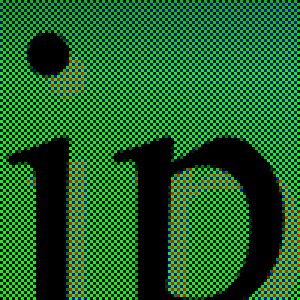
\includegraphics[width=0.2\textwidth]{figures/bayer_frame.png}
        \label{fig:bayer_full}
    }
    \qquad
    \subfloat[Final image]{
        
\includegraphics[width=0.2\textwidth]{figures/bayer_final}
        \label{fig:bayer_final}
    }
    \qquad
    \subfloat[Bayer pattern]{
        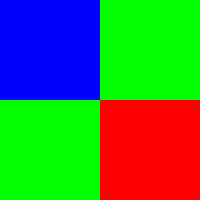
\includegraphics[width=0.2\textwidth]{figures/bayerpattern.png}
        \label{fig:bayer_pattern}
    }

    \caption[Bayer demosaicing]{Bayer demosaicing, \textit{source: https://en.wikipedia.org/wiki/Demosaicing}}
    \label{fig:bayer_channels}
\end{figure}

\begin{enumerate}
    \item Receive raw sensor data, often a Bayer image or similar. A Bayer
        image is constructed using two green channels, one red, and one blue as
        seen in \cref{fig:bayer_pattern}. Like mentioned in \cref{section:imageformats},
        the human eye sees more green than other colors, so the pattern has
        more green than red and blue. There are other similar formats, though
        they all work more or less in the same way.

    \item The ISP then begins applying the autocontrol algorithms, the standard
        ones are known as the \textit{Triple Autocontrol} (3A) algorithms for
        auto white balancing, gain/exposure, and focus control~\cite{libcameraStack}.
        These will be covered in a bit more detail in
        \cref{section:autocontrol}.

    \item Apply other autocontrol algorithms, the specifics will be covered later.

    \item Demosaic the image, i.e., extracting the pixel data from the raw
        image. Often done using a Bayer like filter, many exist though
        they all work in the same way. In \cref{fig:bayer_channels} we can see
        how each of these channels are extracted. Once extracted they are
        combined into the final image as seen in \cref{fig:bayer_final}~\cite{li2008image, libcameraStack}. One
        way this can be done is taking the average of each nearby pixel and
        interpolating them into a single one. This is quite crude compared to
        the real thing but the idea is the same.

    \item After processing the image in the ISP, the ISP then gives the image
        to the application that requested the image. The ISP also re-calibrates
        the autocontrol parameters based on the ones that were computed for the
        current frame. This is in order to correct for example white balancing,
        if coming from a very dark room into a very light room, it uses the
        current parameters to improve the white balancing.

\end{enumerate}

\subsubsection{Autocontrol algorithms} \label{section:autocontrol}
When people talk about their images being unedited, most do not realize that all
photos are edited to a degree. Some better than others; autocontrol algorithms
today can process an image quite heavily. This section will give an overview of
what autocontrol algorithms are, covering the basic ones in a more detailed
manner.

ISPs implement \textit{autocontrol algorithms} often referred to as \textit{3A algorithms} (\textit{Auto
White Balancing} (AWB), \textit{Auto Gain Control} (AGC) and \textit{Auto
Exposure Control} (AEC), and \textit{Auto Focus} (AF)) though encompassing many
other algorithms. When the ISP receives metadata from the sensor, it uses the
AEC and AGC algorithm to increase or decrease the brightness to ensure that the
image will not be too bright or dark. The purpose of AWB on the other hand is
to make sure that the color temperature of the image is correct. Blue being cold and
yellow being warm, it balances the whites to reflect reality as closely as
possible.

\textit{\textbf{Automatic White Balance}} (AWB) ensures that colors appear
natural by adjusting the image so that white objects look white, regardless of
the light source. When humans look at an object, we perceive that the objects color
does not change. In reality, the color does change. Indoors the color
is bluer and outside the color is more orange. Our eyes have over the years
gotten very good at adjusting color differences. This is called \textit{color
consistency}~\cite{foster2011color, ebner2021color}. What AWB tries to do is
mimic the human ability and keep the color consistent. There are a variety of
different approaches to this problem~\cite{agarwal2006overview}, the Pi uses a
Bayesian approach.

\begin{figure}
    \begin{center}
        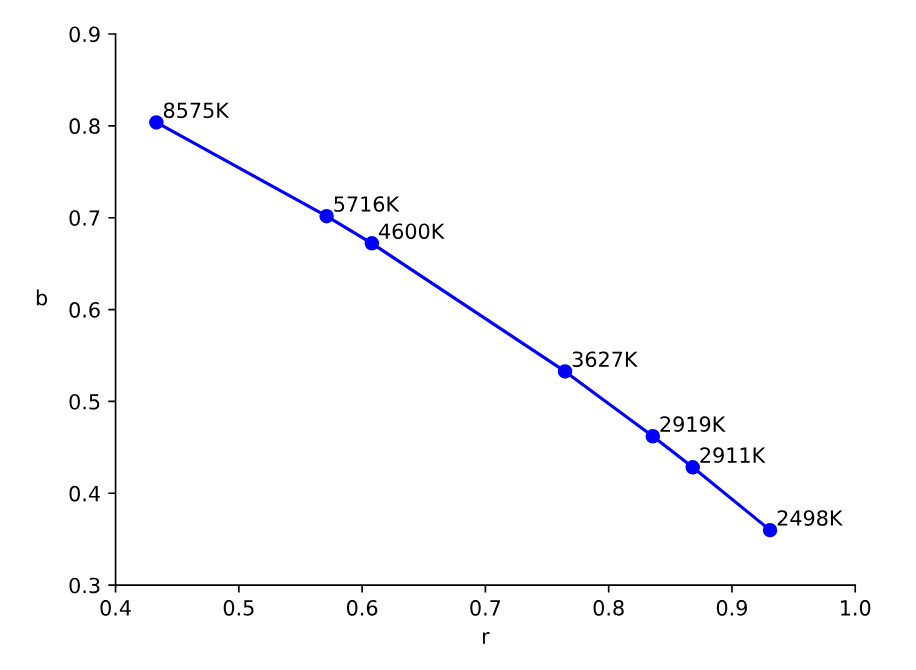
\includegraphics[width=0.4\textwidth]{figures/temperature.png}
    \end{center}
    \caption{Color temperatures with blue and red normalized, \textit{image source: \cref{note:tuningguide}}}\label{fig:temperatures}
\end{figure}
In order to achieve this, one must first tune the AWB algorithm. This is done
through capturing an image of a color checker chart where the colors are known.
For each RGB value that is received, the value is normalized so that $r = R /
G$ and $b = B / G$. When these are plotted we get a \textit{Color Temperature
Curve} (CT curve) as seen in \cref{fig:temperatures}. This CT Curve
represents the \textit{Planckian Locus}
temperature curve which can be used to estimate the temperature of a color that
is output by a \textit{Planckian Radiator}~\cite{international1957international}.
A Planckian Radiator is almost any object that outputs light through heat,
however with LEDs this is not exactly true. The Bayesian theorem is then used
to find the most probable temperature in this curve. Once the most probable
color temperature has been determined, the AWB algorithm then applies gain to
the red and blue color channels to get to the desired temperature.

\textit{\textbf{Auto Focus}} (AF)  adds automatic focusing on objects. While
one of the 3As, AF is not always available depending on the camera module, these
cameras are called \textit{fixed focus cameras}. For AF to exist, it needs a way to move
the lense, this is often done with a \textit{Voice-Coil Motor}~\cite{coilmotor2007}.
This adds complexity to the camera, which depending on your use case might not be
necessary as well as additional points of failure.

In general autofocus can be categorized into two different approaches: active
and passive. The active approach is similar to how 3D cameras work
(see~\cref{section:3Dcameras}) where a laser can be fired to measure distance
or something similar. Passive on the other hand uses \textit{Phase Detection
Auto Focus} (PDAF) or \textit{Contrast Detection Auto Focus} (CDAF).

\begin{figure}
    \centering
        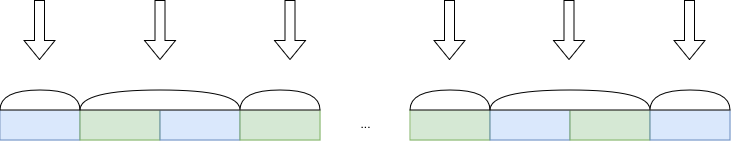
\includegraphics[width=0.7\textwidth]{figures/pdaf_sensor.png}
        \caption{An unfocused microlense PDAF pixel, the left side has a
        different offset than the right.}
        \label{fig:pdaf}
\end{figure}

\pagebreak
\begin{wrapfigure}{r}{0.4\textwidth}
    \begin{center}
        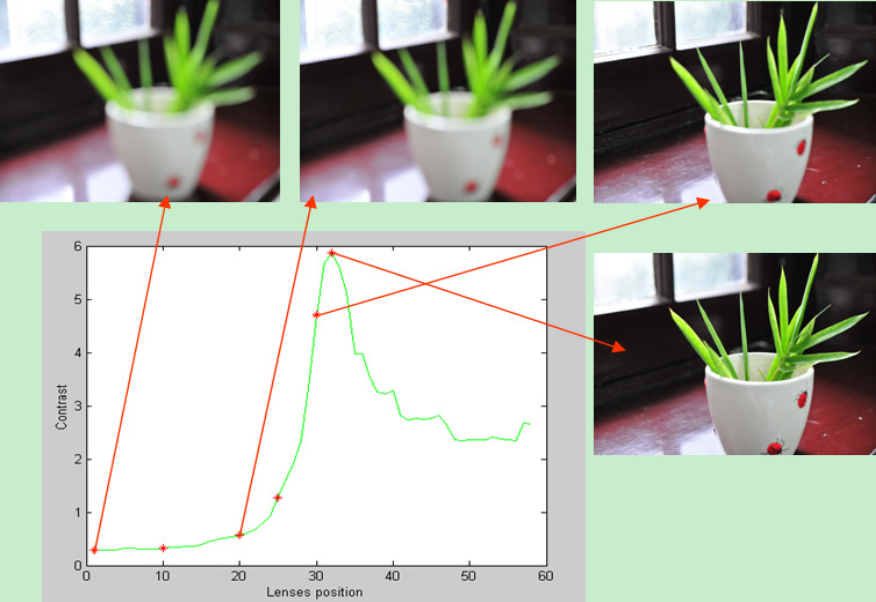
\includegraphics[width=0.35\textwidth]{figures/cdaf.png}
    \end{center}
    \caption{CDAF example~\cite{xu2011robust}}\label{fig:cdaf}
\end{wrapfigure}
PDAF is similar to how stereo cameras covered in \cref{section:3Dcameras}
work. It uses a pair of "image views" (in reality, there are multiple of these pairs)
looking for, as the name suggests, phases. While a phase is slightly
misleading, what it means is that the sensor looks for objects that have some
horizontal gradient. Objects such as a vertical grating have very large
gradients and serve the purpose very well, though it can look for it in
anything. These gradients are viewed through two PDAF sensors like in
\cref{fig:pdaf}. The "large" microlense above the pixel bends the light coming
in so that each pixel sees either the left or right side of the
lens\footnote{This is but one implementation, some systems can use "shielded"
pixels as to block a part of the light.}. They then compare the offset of the
gradient to see if it is the same on both sides. An image of a vertical
grating for example would have shifts in it, though very small if unfocused~\cite{pdafPatent}.
This then provides a weight for the AF algorithm to adjust the focus with.

CDAF as the name suggests analyses the contrast of an image to adjust the
focus. The contrast of an image increases as the image comes into focus~\cite{xu2011robust}.
An example of this can be seen in \cref{fig:cdaf} where the contrast rapidly
increases as it comes into focus, only to rapidly drop once it is out of focus.
CDAF has a drawback though, if the focus window is too large it can be difficult
to find a focus. This is due to the background having such a large part of the
focus window. A workaround for this is to focus on a smaller area.

\textit{\textbf{Automatic Gain Control}} (AGC) and \textit{\textbf{Automatic
Exposure Control}} (AEC) work in tandem to optimize image brightness and
contrast. They control exposure settings by dividing the image into regions to
calculate an average luminance value, which is then compared against a target
value. The algorithm uses histogram analysis to ensure that highlights are not
overexposed and shadows are not underexposed. Adjustments are made to shutter
speed and sensor gain to reach the desired exposure level while maintaining
image quality.

The Raspberry Pi first calculates the weighted average luminance, it does this
by diving an image into 16x16 regions which have weights assigned to them. The
average is then calculated using the following formula:~\[Y = \frac{\sum_{i \in \text{regions}} w_i Y_i}{\sum_{i \in \text{regions}} w_i}\]

\begin{wrapfigure}{l}{0.5\textwidth}
    \centering
    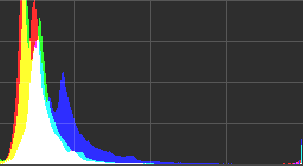
\includegraphics[width=0.48\textwidth]{figures/histogram.png}
    \caption{Intensity histogram taken from an image edited in Krita}
    \label{fig:intensityhistogram}
\end{wrapfigure}
Intensity histograms represent how much of each color there is on an image. In
\cref{fig:intensityhistogram} we can see an example of an intensity histogram,
if the image would have been a gray scale, there would of course only have been
one channel. This histogram is built by iterating through each pixel in the
image, counting the channel intensity for each color. The white histogram
represents brightness. One way to compute the brightness of a pixel is $Y = (R
+ G + B) / 3$, which is a trivial way, a better implementation can be found
here~\cite{kumar2010theory}.

The Pi creates a \textit{Cumulative Frequency Function} (CFA) $F(p)$ of the brightnesses which
is normalized so that it 0 represents no pixels and 1 represents all pixels are
below $p$. \textit{Quantiles} represent a point in the CFA where all pixels are
below a given proportion $p = Q(q)$. This breaks if $Q$ is not single valued,
for example in cases where the image is black and white, such as an image of
a book. To fix this, the Pi computes an inter-quantile mean
$I(q_0, q_1) = Y_{target}$. For example $I(0.75, 1) = 0.5$ means that we want
the top 25\% of the histogram to be above the 0.5 pixel range. In order to
achieve this, the ISP adjusts the exposure time and digital gain levels with
small increments until it is reached.

On top of the 3A algorithms, there are a lot more that the ISP often does. For
example there is often some vignette, color correction and more. In
\cref{fig:lens_shading} we can see an example of how the ISP has fixed the image.
In \cref{fig:with_shading} the corners are significantly darker than the center,
while in \cref{fig:without_shading} the whole image is equally lit. An image
may also have the colors slightly (or a lot) wrong. It can then compute the
histograms for each color, and try to balance the colors. We can see an example
of this done in software in \cref{fig:nocolorcorrection} where the image is
very green. After balancing the colors in \cref{fig:colorcorrection} the image
looks normal once more. There are many more processing algorithms that are run
on the images, for a more thorough overview of each of these please refer to
the Pi ISP specification\footnote{https://datasheets.raspberrypi.com/camera/raspberry-pi-image-signal-processor-specification.pdf}.

\begin{figure}[htpb]
    \centering
    \subfloat[With vignette]{
        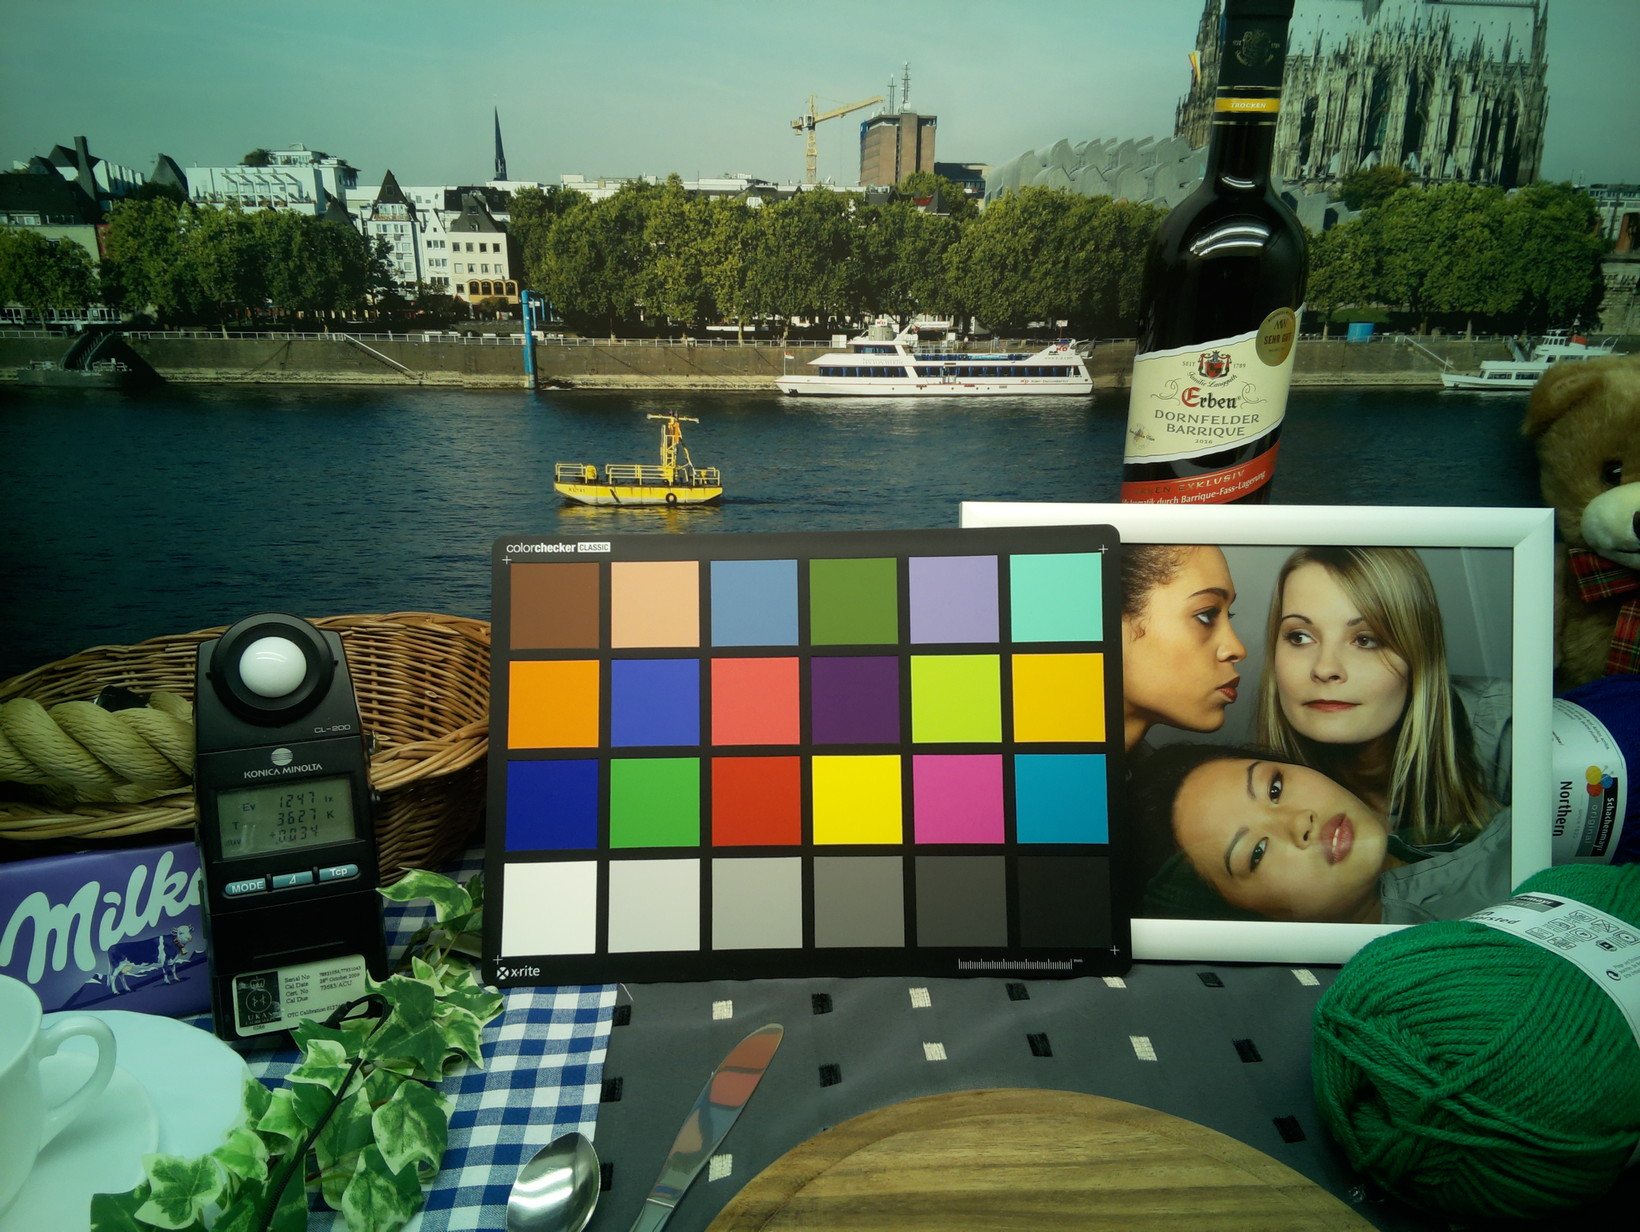
\includegraphics[width=0.35\textwidth]{figures/alsc-none.jpg}
        \label{fig:with_shading}
    }
    \subfloat[Without vignette]{
        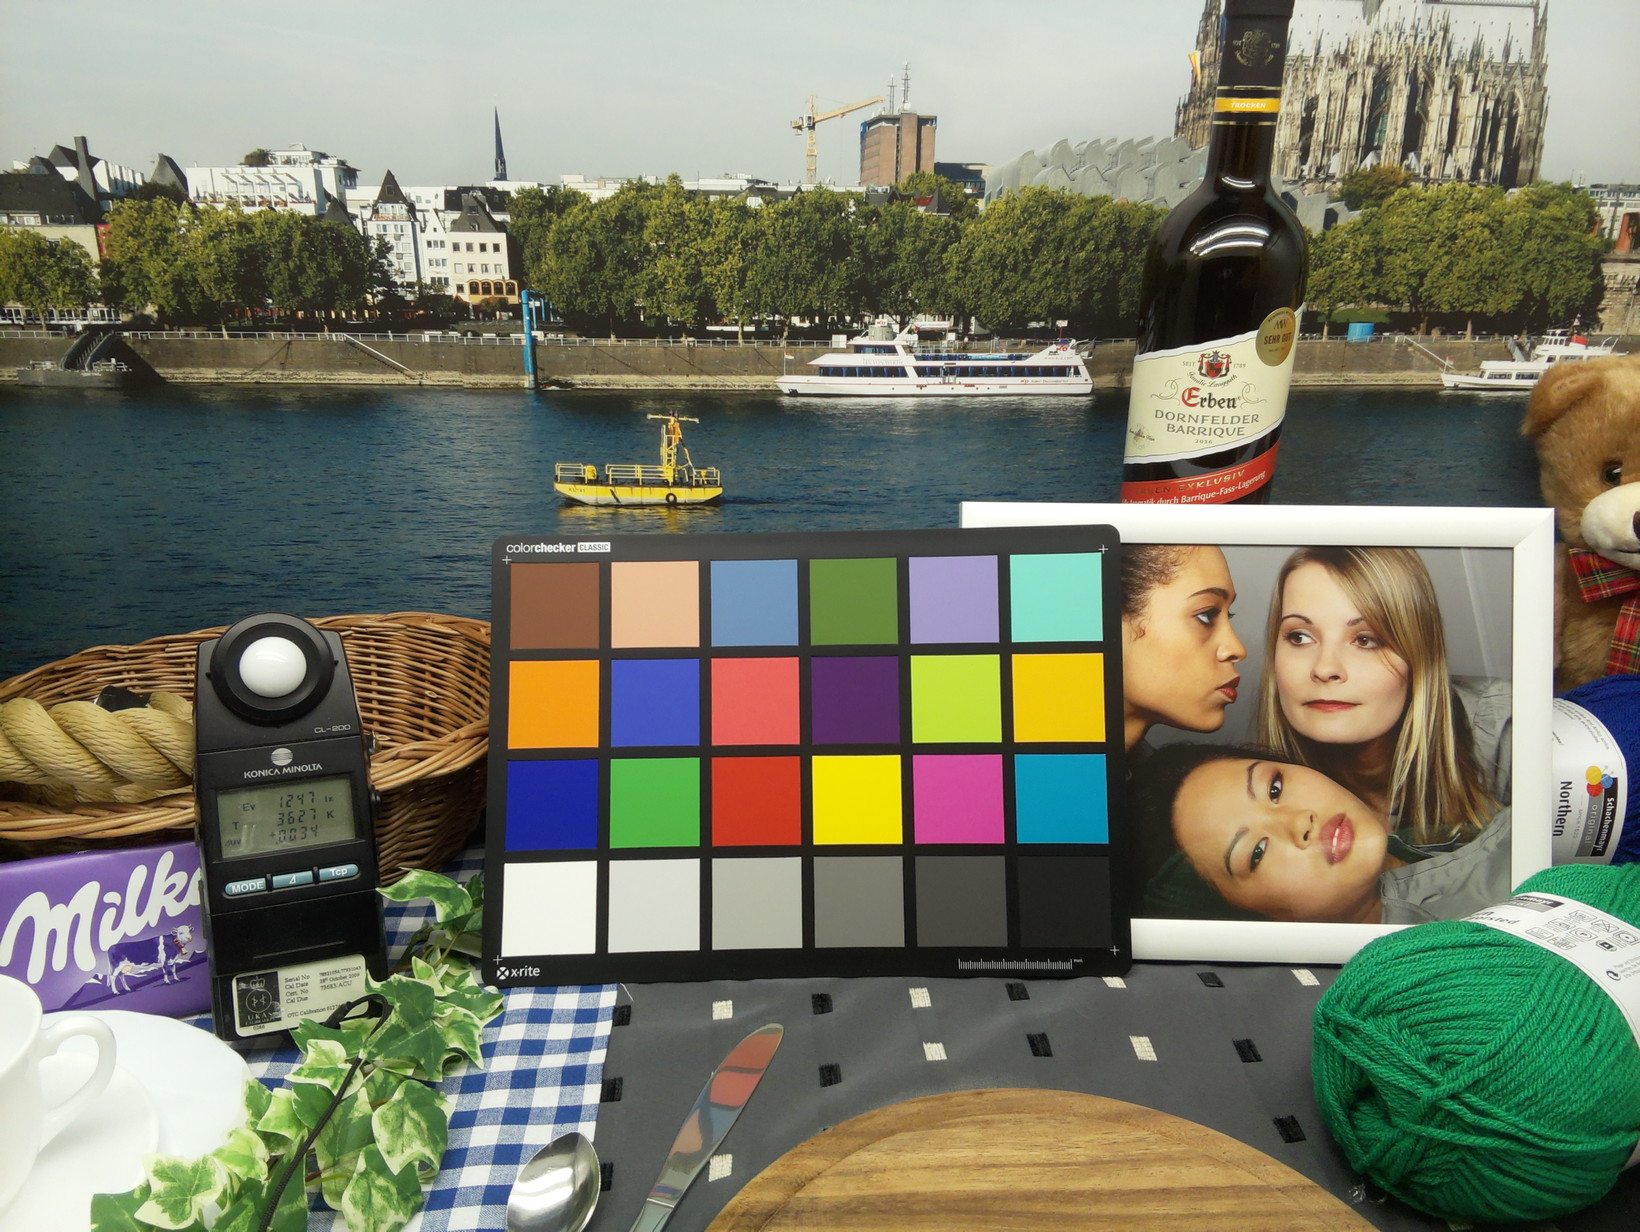
\includegraphics[width=0.35\textwidth]{figures/alsc-both.jpg}
        \label{fig:without_shading}
    }
    \qquad
    \subfloat[Without color correction]{
        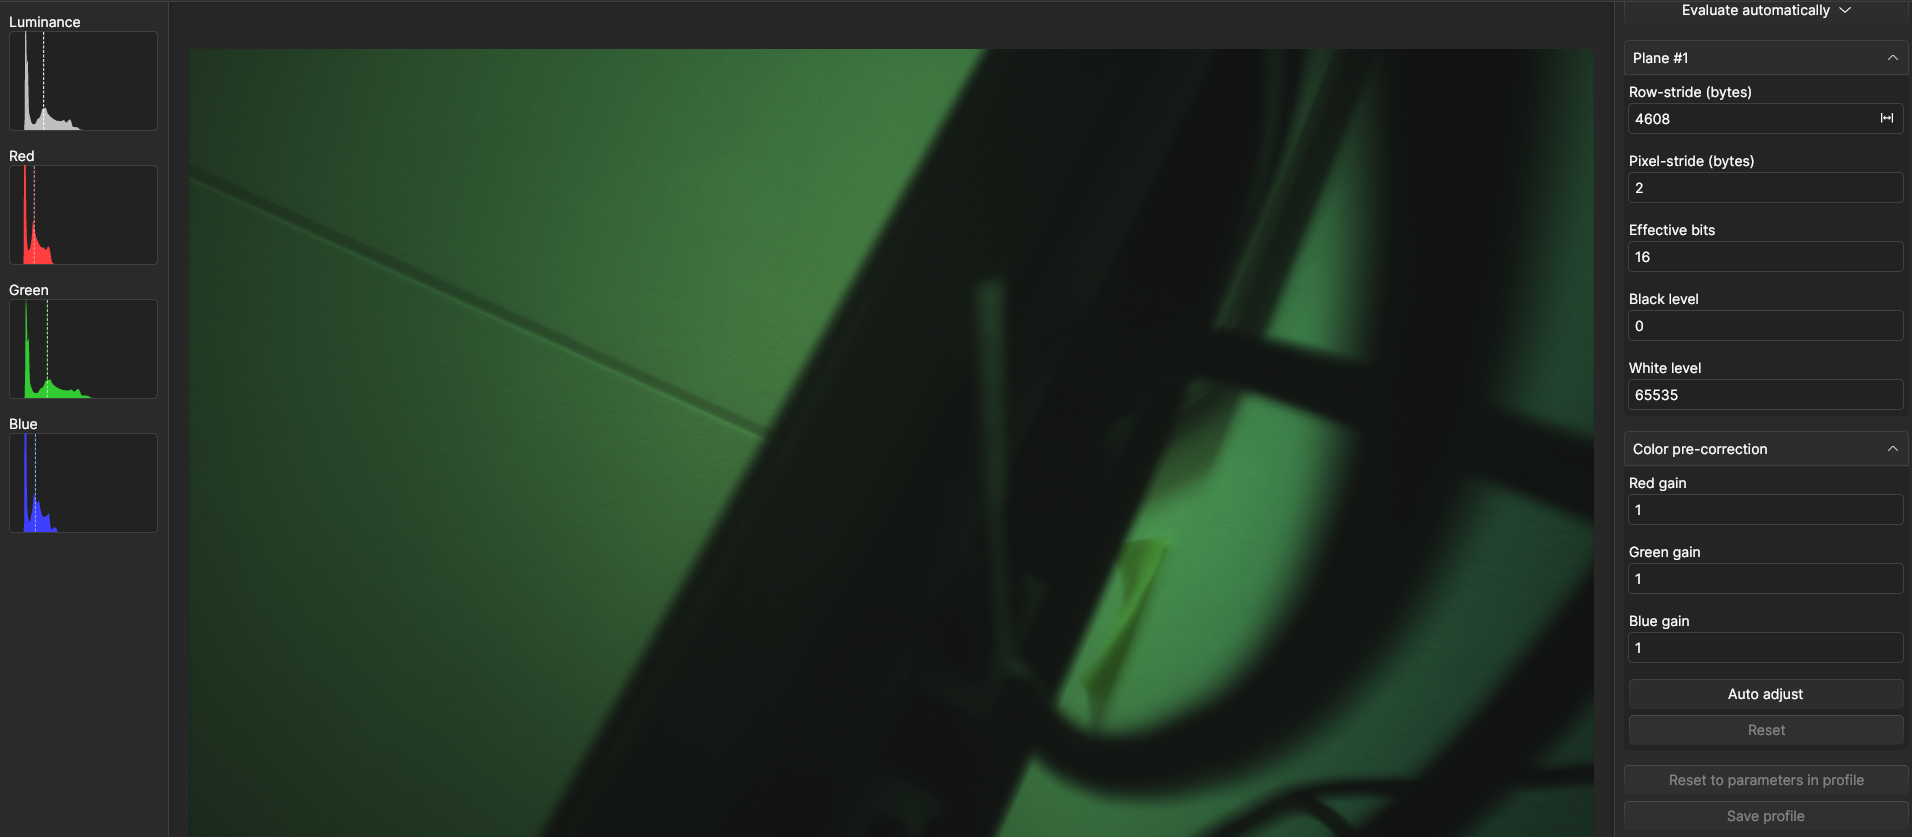
\includegraphics[width=0.5\textwidth]{figures/nocolorcorrection.png}
        \label{fig:nocolorcorrection}
    }
    \subfloat[With color correction]{
        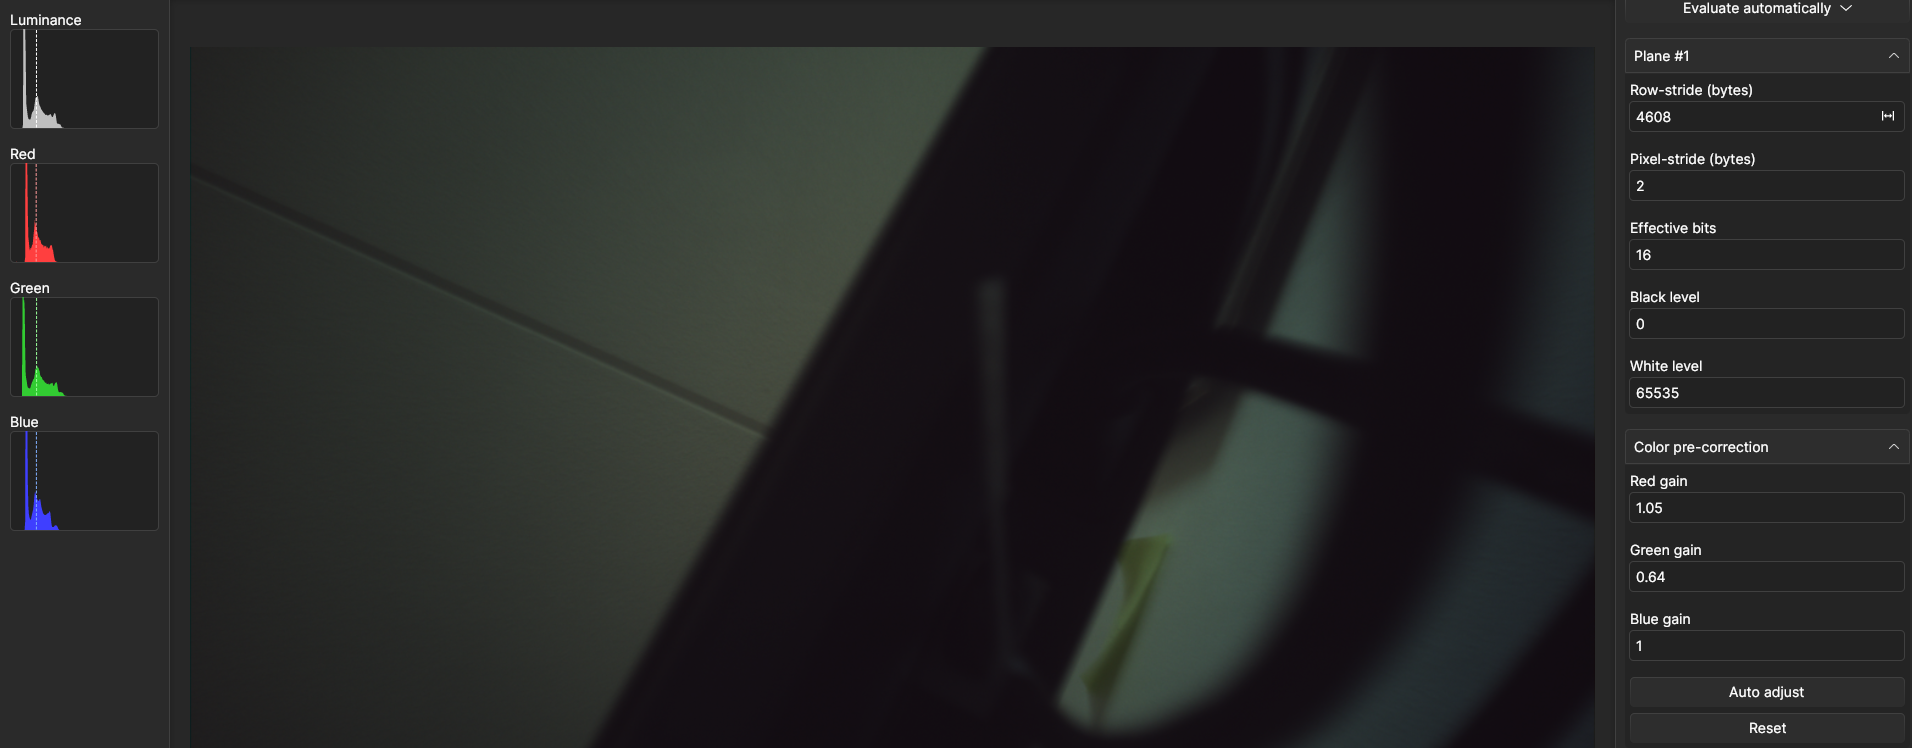
\includegraphics[width=0.5\textwidth]{figures/colorcorrection.png}
        \label{fig:colorcorrection}
    }

    \caption{Different vignette corrections. \textit{Photo by Naushir Patuk used with permission}}\label{fig:lens_shading}
\end{figure}

\subsubsection{Image Processing and Tiles}
The Raspberry Pi ISP is divided into two sections, the front- and back end.
While the front end has some image processing capabilities, being able to scale
and crop images, its main responsibility is to write images to main memory.
It provides an AXI\footnote{https://developer.arm.com/documentation/ihi0051/latest}
interface to give the ISP frames. While doing this, it provides the backend
with some statistics of the image. These statistics consist of for example
histograms of color counts etc.

The backend then reads these images that the frontend has provided. Unlike how
applications deal with full frames, the backend deals with \textit{tiles}. The
Raspberry Pi uses tiles that are 640x640 aligned to 64 bits. This is done in
order to reduce the amount of memory required to process an image and speed up
memory access. By limiting it to tiles of the image, significantly less memory
is required for a 4K image to be processed. Additionally this means that the
image processing can be parallelized, by splitting the image into several
chunks the ISP can safely process the image in parallel.


\subsection{CSI-2}
\begin{figure}
    \begin{center}
        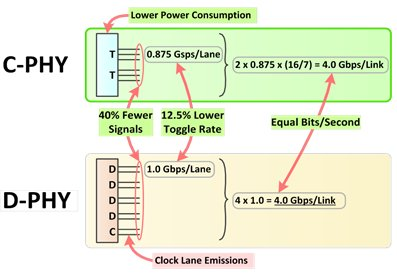
\includegraphics[width=0.55\textwidth]{figures/cphydphy.jpg}
    \end{center}
    \caption{A comparison of C-PHY vs D-PHY, \textit{image source: \href{https://www.design-reuse.com/articles/43954/demystifying-mipi-c-phy-dphy-subsystem.html}{demystifying mipi c phy dphy subsystem}}}
    \label{fig:cphydphycomparison}
\end{figure}

CSI-2\footnote{https://www.mipi.org/specifications/csi-2} is a technology to
transport sensor data over short distances very quickly. While being initially
made for mobile, the technology has moved to automotive. As CSI-2 initially was designed for
mobile devices, it is not made to transport data over long distances. This has made it
slightly more difficult in the automotive industry, as cars are larger than a
few centimeters. The solution for this is often to have another technology such
as GMSL\footnote{https://www.analog.com/en/solutions/gigabit-mulitimedia-serial-link.html}
though as long as there is enough bandwidth the data could even be converted to
an IP packet. Once it is within range, it is converted back to CSI-2.

CSI-2 uses two different technologies, namely C-PHY and D-PHY. These can
transport data at different speeds. Along with the fast C-PHY/D-PHY lanes,
control lanes are also provided that control the camera over I$^2$C. Each API
can be used on the same chip, if speed is needed C-PHY should be used. While
D-PHY is much simpler to implement as it is a basic master/slave system similar
to I$^2$C.

D-PHY uses a dedicated lane for clock, this means that it only has two lanes for
data transport. It is a very simple synchronous protocol, it does not encode the
bits in any way.

Unlike D-PHY, C-PHY does not have a dedicated lane for clock. It uses all lanes
for both clock and data transport, embedding the clock implicitly into the
data. C-PHY encodes the bits into symbols, the encoder then guarantees that
there will be at least one edge in the signal. This allows the receiver to
derive a clock. Encoding the data, allows one to pass more information to the
receiver at once opposed to if no encoding would be done.

C-PHY works in the following way, it always uses triplets of cables. The spec
does not allow for the voltage in all three cables to be either positive or
negative. This means that we are left with 6 combinations the cables can be in.
The data bits are not directly derived from the polarities, instead they are
decoded from the "moves" from one state to another. These symbols are often
sent in groups of 7, into these 7 symbols 16 bits\footnote{16 bits is a nice
amount, it fits on 2 lanes and is easily parallelizable} are encoded\footnote{\href{https://www.mipi.org/specifications/c-phy}{MIPI C-PHY spec}}.

CSI-2 is often used where speed is crucial, if the symbol rate is 2 Giga symbols per second (Gsps),
it follows that the bit rate for each triplet is
$(16\text{bits} / 7\text{symbols}) * 2\text{Gsps} = 4.57 \text{GBps}$.
In \cref{fig:cphydphycomparison} we can see how the two technologies compare,
with D-PHY we need much more connections compared to C-PHY to reach the same
speed.

\subsection{I2C}
\textit{Inter-Integrated Circuit} (I2C) is a widely used standard\footnote{\href{http://www.nxp.com/docs/en/user-guide/UM10204.pdf}{https://web.archive.org/web/20221006073143/http://www.nxp.com/docs/en/user-guide/UM10204.pdf}}
in configuring cameras today. It is based on the
master/slave system where the master controls the clock, sending signals to the
slave device which responds whenever addressed. A host computer for example
configures camera devices. I2C is a two wire system with a clock wire and a
data wire\footnote{\href{https://patents.google.com/patent/US4689740A/en}{https://patents.google.com/patent/US4689740A/en}}
where after each clock pulse the data wire can change.

\begin{figure}
    \begin{center}
        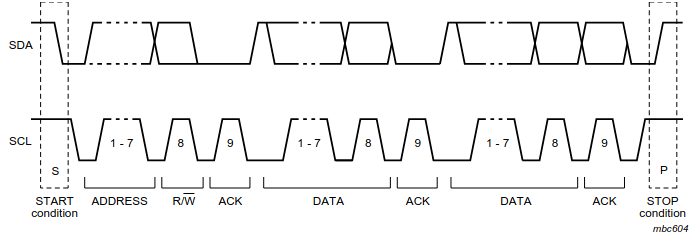
\includegraphics[width=0.95\textwidth]{figures/I2C_transaction.png}
    \end{center}
    \caption{I2C Communication transaction, SCL is the clock lane and SDA is the data lane.
        \textit{Image source: \href{https://www.nxp.com/docs/en/user-guide/UM10204.pdf}{https://www.nxp.com/docs/en/user-guide/UM10204.pdf}}}\label{fig:I2C}
\end{figure}

The communication process works in the following way as seen in \cref{fig:I2C}:

\begin{enumerate}
    \item The master initiates the communication by lowering the data lane and
        keeping the clock lane up.

    \item The master sends a 7-bit address through the data lane to specify
        which device it wants to communicate with, followed by a read or write
        bit specifying which operation it wants to do.

    \item After receiving the message, the slave acknowledges (ACK) that it received
        the message by pulling down the data lane. If it is not ready, it will
        leave the data lane up (NAK).

    \item When the slave has responded, the master will send the data in 8-bit
        frames followed by an ACK/NAK bit.

    \item The transfer is finally stopped by releasing the data lane while the
        clock lane is up.
\end{enumerate}

In userspace Linux I2C is configured using \textit{ioctl} commands. This will
briefly be covered in \cref{section:v4l2}.

\section{History}
In the early days cameras were quite simple, there effectively was just a
function to tell the camera to capture an image. This process did not allow for
much customization. This was the case with most cameras such as webcameras where
the camera sensors were "smart sensors". This means that the cameras had a
small ISP integrated into them, they could do the image processing internally. Even
the integrated laptop ones were just USB devices that output images in a
similar fashion. Linux had initially had lacking support for this, but in the
late 1990s Video For Linux (V4L, later V4L2 for version 2) was developed. This
covered most of the use cases at the time.

Over the years V4L had grown organically, developing features on the fly as
they were needed. This meant that there was no large plan being executed, in
turn the design turned out to be far from optimal\footnote{Direct documentation
on what was wrong with the API has not really been written, this is based
on a discussion with Laurent Pitchard}. In 1998 Bill Dericks began the
design and development of V4L2 which we have in use today\footnote{https://www.kernel.org/doc/html/v4.9/media/uapi/v4l/hist-v4l2.html}.
V4L2 got merged into Linux 2.5.x/2.6 (around 2003), deprecating the
original one.

\begin{figure}
    \centering
    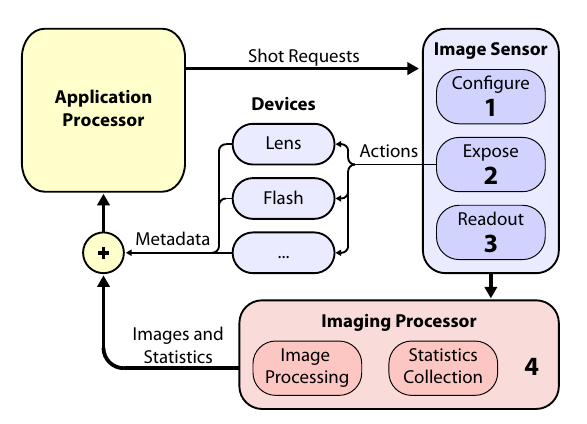
\includegraphics[width=0.48\textwidth]{figures/fcam_arch.png}
    \caption{Frankencamera architecture~\cite{adams2010frankencamera}}
    \label{fig:fcam_api}
\end{figure}

In 2009 the Nokia N900 was released, this was a Linux based phone that included a camera that was not
like most cameras at the time. It provided interfaces for customizing just
about everything. From ISPs to Image Processing Algorithms (IPAs), this meant
that the current way camera APIs worked was no longer maintainable. It
required that the application would manage everything, computing the
histograms, configuring the autocontrol etc. While this was doable for a
company on the scale of Nokia at the time, it was not for anyone else. Enter
Frankencamera~\cite{adams2010frankencamera}; this was an effort at the time
to create an API that allowed the user to express the different options that
cameras needed. This effort was lead by Stanford and Nokia, it is what most
modern APIs are based on at a high level. It was built on top of V4L2,
providing a more user friendly API.

Like its successors covered in~\cref{section:currentAPIs}, the Frankencamera API
was a request based API. The idea with it was to allow for the user to control
the cameras very well. \cref{fig:fcam_api} shows the block diagram of how the
API worked. The application would request a capture, the sensor gets
reconfigured based on the request. After which it would capture the image with
which ever peripherals the user has and finally forward the image to the ISP.
The ISP then processes the image and gives it to the application along with the
metadata. This will look very similar to how modern APIs work which is covered
in~\cref{section:currentAPIs}.

Before Frankencamera many camera APIs were stateful~\cite{experimentalCompPhot},
they only had one state that controlled the sensor. This meant that when you
wanted to capture multiple images with multiple settings the changes would take
effect at an unpredictable time in the future. While also adding latency to
manage the state internally, it also meant that you had to clear the capture
pipeline so that you could guarantee that the settings were correct. This was a
very complex process, though state was important; it was placed in the wrong
place. This lead to the creation of the request based API, where the
application would manage the state and the camera would simply accept requests.
